\documentclass[sigconf]{acmart}

\usepackage{booktabs} % For formal tables
\settopmatter{printacmref=false}



% Copyright
%\setcopyright{none}
%\setcopyright{acmcopyright}
%\setcopyright{acmlicensed}
\setcopyright{rightsretained}
%\setcopyright{usgov}
%\setcopyright{usgovmixed}
%\setcopyright{cagov}
%\setcopyright{cagovmixed}


% DOI
\acmDOI{10.475/123_4}

% ISBN
\acmISBN{123-4567-24-567/08/06}

%Conference
%\acmConference[WOODSTOCK'97]{ACM Woodstock conference}{July 1997}{El  Paso, Texas USA} 
%\acmYear{1997}
%\copyrightyear{2016}


%\acmArticle{4}
%\acmPrice{15.00}

% These commands are optional
%\acmBooktitle{Transactions of the ACM Woodstock conference}


\begin{document}
\begin{titlepage}
\title{%\vspace{-1cm}
Speeding up  Children Reunification in Disaster \\ Scenarios via Serverless Computing\textsuperscript{1}} 
\subtitle{Extended Abstract}
%\subtitlenote{}


\copyrightyear{2017} 
\acmYear{2017} 
\setcopyright{acmcopyright}
\acmConference[WoSC'17]{WoSC'17: Workshop on Serverless Computing}{December 11--15, 2017}{Las Vegas, NV, USA}
\acmBooktitle{WoSC'17: WoSC'17: Workshop on Serverless Computing, December 11--15, 2017, Las Vegas, NV, USA}
\acmPrice{15.00}
\acmDOI{10.1145/3154847.3154851}
\acmISBN{978-1-4503-5434-9/17/12}


\author{Kyle Coleman}
\orcid{1234-5678-9012}
\affiliation{%
  \institution{Computer Science Department}
  \city{Saint Louis University, St. Louis, MO} 
  \state{} 
%  \postcode{43017-6221}
}
\email{kyle.coleman@slu.edu}




\author{Flavio Esposito}
\orcid{1234-5678-9012}
\affiliation{%
  \institution{Computer Science Department}
  \city{Saint Louis University, St. Louis, MO} 
  \state{} 
%  \postcode{43017-6221}
}
\email{flavio.esposito.slu.edu}

\author{Rachel Charney}
\orcid{1234-5678-9012}
\affiliation{%
  \institution{Department of Pediatrics}
  \city{Saint Louis University, St. Louis, MO} 
  \state{} 
%  \postcode{43017-6221}
}
\email{rachel.charney@health.slu.edu}



\begin{abstract}
Children constitute a vulnerable population and special considerations are necessary in order to provide proper care for them during disasters. After disasters such as Hurricane Katrina, the rapid identification and protection of separated children and their reunification with legal guardians is necessary to minimize secondary injuries ($i.e.$, physical and sexual abuse, neglect and abduction). At Camp Gruber, an Oklahoma shelter for Louisianan's displaced by Hurricane Katrina, $70\%$ of the children were with their legal guardian after 2 weeks while the last child was reunified after 6 months. 

In this project, we are using serverless computing to scale and minimize database querie response time as well as to speed up machine learning tasks for rapid reunifying time, in support of a federated set of first-responders. In particular, we are using a Flask-based web system that leverages Apache OpenWhisk to run both (face and text) profile recognition software at the back-end.
\end{abstract}



%
% The code below should be generated by the tool at
% http://dl.acm.org/ccs.cfm
% Please copy and paste the code instead of the example below. 
%


\maketitle
\section{Introduction}
\label{sec:intro}

\vspace*{-4pt}
Large scale natural disasters such as Hurricane Irma result in insurmountable damage to structures and devastating chaos within families. Many children are separated from their families and reunification can be a time and resource-consuming challenge. Distressed, young or injured children often cannot self-identify. Examples of text features used for recognition by first-responders are  name, home address, and social security number. Matching this information manually (when available) can prolong the reunification time. 
%
To solve this problem, we are prototyping a system empowered by serverless computing for fast, scalable and federated (children) profile matching. 
%
\begin{comment}
Serverless computing has erupted with the emergence of several commercial platforms, $e.g.$, Amazon's AWS Lambda, Google Cloud Functions, Microsoft's Azure Functions, and the open-source counterparts, $e.g.$, OpenLambda~\cite{lambda} and IBM's OpenWhisk~\cite{openwhisk}. 
\end{comment}

In serverless computing, the application logic is split into functions called by external or internal events. 
%
The actions in our case are defined by machine learning (classification) operations. In particular, the system goal is to match text and visual profile information, uploaded by guardians, with children's profiles available on the distributed database.  Our events instead are database queries executed by first-responder devices.
%
\vspace*{-1mm}
\begin{figure}[t]
\begin{center}
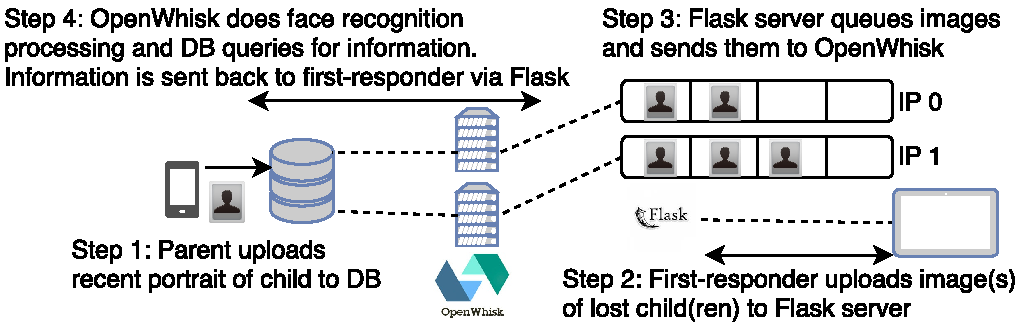
\includegraphics[width=75mm, scale=1]{framework.pdf}
\vspace*{-5mm}
\caption{\footnotesize{System Architecture and workflow}
%\footnotesize{Guardians upload images to our Flask server. The Flask server groups incoming images based on the IP of the sender. This allows us to  track senders. Upon first responders requests, we then send these groups of images to our OpenWhisk framework for database processing and match retrieval.}
}
\label{figure1}
\end{center}
\vspace*{-6mm}
\end{figure}
%\vspace*{-6mm}
%
We use serverless computing to inherit the benefits of an idle but responsive platform in case of bursty demands, common in emergency situations such as a natural disaster.
Our prototype utilizes specifically Apache OpenWhisk~\cite{openwhisk}.
%
In the next section we describe our system design and our ongoing work.
%\vspace*{-2pt}

%---------------------------------------------------------------------------------------------

%\vspace*{-4mm}
\section{System Architecture}
\label{sec:frame}
%\vspace*{-2pt}

%----------------------------------------------
%\begin{comment}
%\end{}
%\end{comment}
%----------------------------------------------
\vspace*{-4pt}
Our prototype utilizes serverless computing in conjunction with Flask ~\cite{flask}, an efficient micro-framework for web development.

A user with a mobile device requests a profile match via a HTTP POST that uploads images to our Flask web server, which  pre-processes by queuing the images based on the unique IP address of the sender. After the collected images are uploaded, they are forwarded to our Apache OpenWhisk server. Here, we run a face recognition application, available at~\cite{ageitgey}.  

We are extending our system so that the application will compare both text and existing uploaded photos against a pre-existing collection of profiles. When a match is found, the system will utilize the name attached to the pre-existing photo to perform a database query for relevant information regarding the child. The database will then return identifying information such as Date of Birth, Social Security Number, emergency contact information, current medications, existing health problems such as allergies, and medical history in an easily readable format. We will test our system using anonymized images and profiles available from the Disaster Preparedness Center at SSM Cardinal Glennon Children's Hospital.

Our system usage will be easily extendable to other types of missing scenarios, for example, adults, elderly or handicapped patients, or even pets. Our system design is general enough and a good proof-of-concept demonstrating how to apply serverless technology to a useful set of delay sensitive applications by means of machine learning tools.


\footnotetext[1]{This work has been supported by the National Science Foundation award CNS-1647084.}
\bibliographystyle{ACM-Reference-Format}
\bibliography{refs} 
\end{titlepage}
\end{document}
